\documentclass[11pt]{beamer}

\usetheme{Rochester}
\definecolor{UBCblue}{rgb}{0.04706, 0.13725, 0.26667} % UBC Blue (primary)
\usecolortheme[named=UBCblue]{structure}

\usepackage[utf8]{inputenc}

\usepackage[english]{babel}

\usepackage{amsmath}
\usepackage{amsfonts}
\usepackage{amssymb}
\usepackage{graphicx}
\DeclareMathOperator {\argmin}{argmin}

\author{\small Jakob Pirs (XX-XXX-XX, jakob.pirs@uzh.ch)\\
Nina Erminia Cantoni (17-709-221, ninaerminia.cantoni@uzh.ch)\\
Rohit Koonireddy (XX-XXX-XX, rohit.koonireddy@bf.uzh.ch)\\
Yunxiang Guo (XX-XXX-XX, yunxiang.guo@uzh.ch)\\}

\title{Cryptocurrencies and the risk-free rate}


\setbeamertemplate{navigation symbols}{} 

\institute[]{University of Zurich, Department of Banking and Finance} 
\date{\today} 


% ---------------------------------------------------------

\bibliographystyle{apalike} %not used

%\bibliographystyle{abbrv}
%\setbeamertemplate{bibliography item}{\insertbiblabel}

% ---------------------------------------------------------

\begin{document}

\begin{frame}
\titlepage
\end{frame}

% ---------------------------------------------------------

\begin{frame}{Research Question}
 \centering Is there a relationship between cryptocurrencies and the 10 year treasury rate?
\end{frame}

\begin{frame}{Overview}
\tableofcontents 
\end{frame}

% ---------------------------------------------------------

\section{Data}
\begin{frame}{Data}
Through an API we accessed price data from yahoo over a period of 5 years (2018-2022). Finally, the data set comprises:
 \begin{itemize}
        \item 4 crytpocurrencies: \\
        Bitcoin 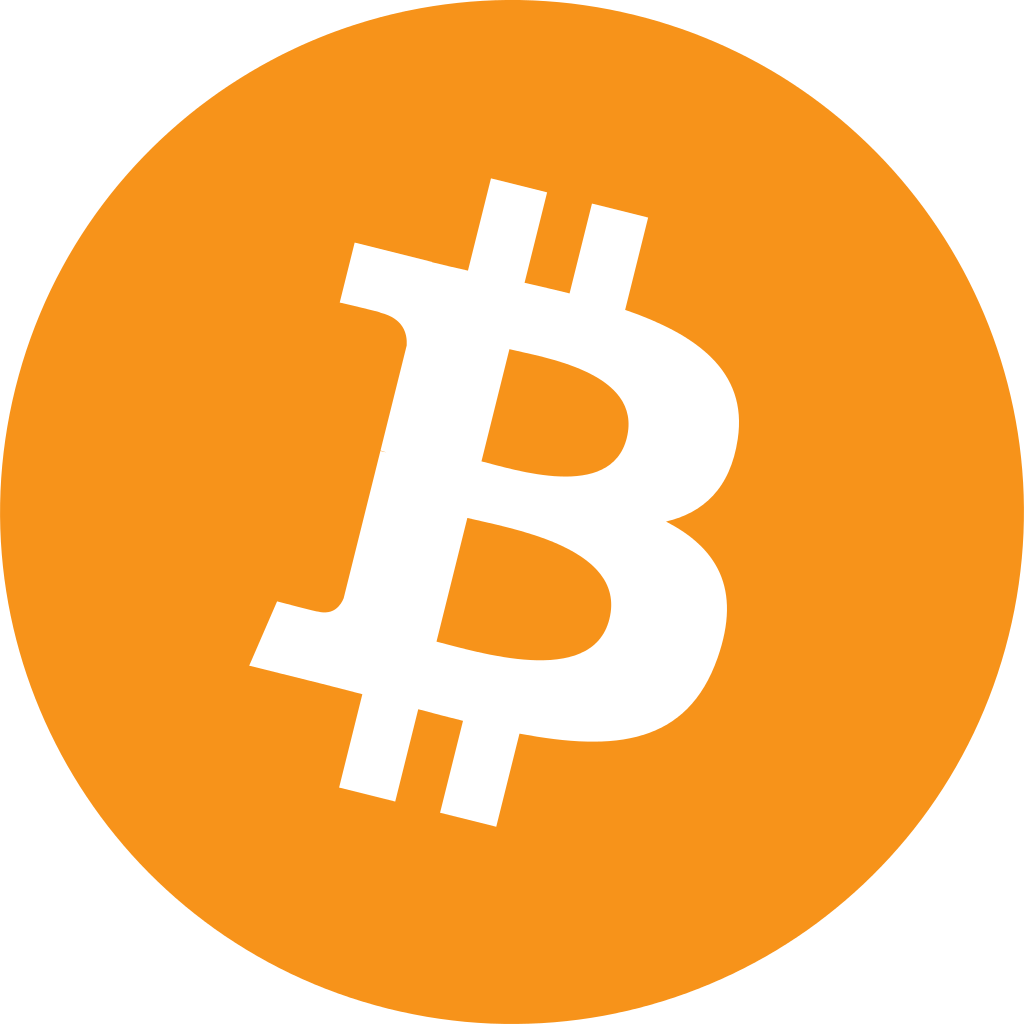
\includegraphics[width=0.05\textwidth]{Bitcoin.png}, Ethereum 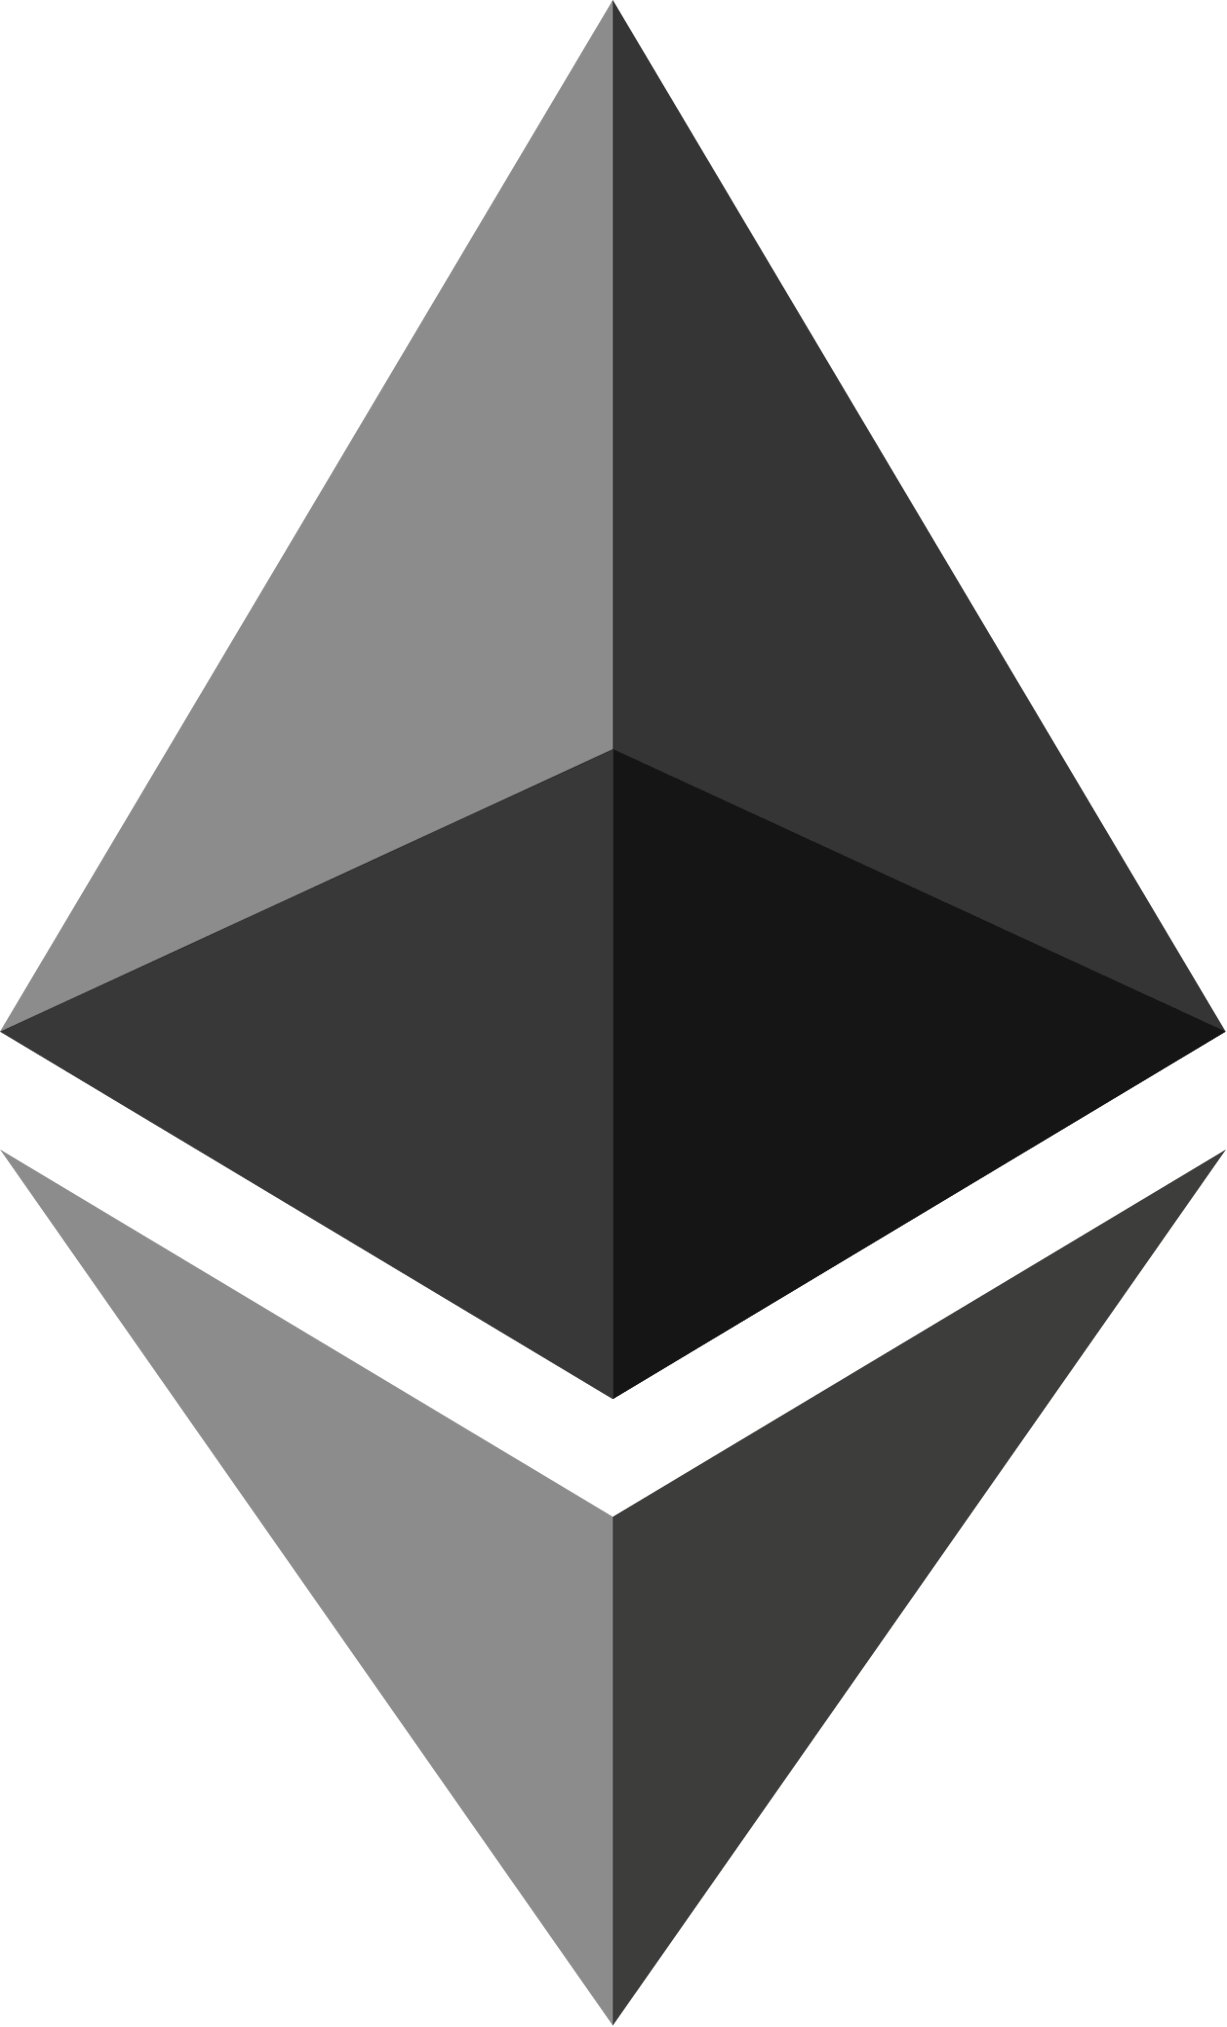
\includegraphics[width=0.035\textwidth]{ETH.png}, XRP 
\includegraphics[width=0.05\textwidth]{XRP.png}, Litecoin 
\includegraphics[width=0.05\textwidth]{LTC.png}
        
        \medskip
        
        \item CMC Crypto 200 Index
        
        \medskip
        
        \item 10 Year US Treasury Rate
    \end{itemize}

\end{frame}

% ---------------------------------------------------------

\section{Methodology}
\begin{frame}{Methodology}
We measure the relationship through:
    
    \begin{enumerate}
        \item Covariance
        \item Pearson's Correlation (linear)
        \item Spearman's Correlation (monotonic)
    \end{enumerate}
\end{frame}

% ---------------------------------------------------------
\section{Results}
\begin{frame}{Results - 1. Covariance}
    tbd
\end{frame}

% ---------------------------------------------------------


\begin{frame}{Results - 2. Pearson’s Correlation (linear)}
    tbd
\end{frame}

% ---------------------------------------------------------

\begin{frame}{Results - 3. Spearman’s Correlation (monotonic)}
    tbd
\end{frame}

% ---------------------------------------------------------

\section{Conclusion}
\begin{frame}{Conclusion}
    tbd
\end{frame}

% ---------------------------------------------------------

\begin{frame}

\begin{center}
    Thank you!
\end{center}

\end{frame}

\end{document}